\documentclass[11pt,oneside,a4paper]{article}
\usepackage{graphicx}
\usepackage{booktabs}
\usepackage{caption}
\usepackage{subcaption}
\usepackage{amsmath}
\usepackage{amsfonts}
\usepackage{amssymb}
\usepackage{lscape}
\usepackage{psfrag}
\usepackage[usenames]{color}
\usepackage{bbm}
\usepackage[update]{epstopdf}
\usepackage[bookmarks,pdfstartview=FitH,a4paper,pdfborder={0 0 0}]{hyperref}
\usepackage{verbatim}
\usepackage{listings}
\usepackage{textcomp}
\usepackage{fancyhdr}
\usepackage{multirow}
\usepackage{tikz}
\usepackage{lipsum}
\usepackage{xcolor}
\usepackage{wrapfig}
\usepackage[margin=1in]{geometry}
\newcommand{\hint}[1]{{\color{blue} \em #1}}

\makeatletter
\def\cleardoublepage{\clearpage\if@twoside \ifodd\c@page\else%
\hbox{}%
\thispagestyle{empty}%
\clearpage%
\if@twocolumn\hbox{}\clearpage\fi\fi\fi}
\makeatother

\sloppy
% \widowpenalty=10000
% \clubpenalty=10000

\title{
    \vspace*{0.0mm}
    \LARGE\bf\sf Advanced Topics in \\Communication Networks (Fall 2019)
    \vspace*{10.0mm} \\
    %
    \Huge\bf\sf Summary
    %
    \vspace*{30.0mm} \\
    \normalsize
    %
    \sf Author:\\[5pt]
    \sf Yannick Merkli\\ [5pt]
    \sf \pageref{lastpage} Pages
}
\date{}

\begin{document}

\maketitle
\thispagestyle{empty}
\raggedbottom
\clearpage

\pagenumbering{roman}

\clearpage
\setcounter{tocdepth}{2}
\tableofcontents
\clearpage
\pagenumbering{arabic}

\section{Introduction}

Networking is on the verge of a paradigm shift towards deep programmability.

\subsection{The network managment crisis}
Networks are large distributed systems running a set of distributed algorithms. These algorithms produce the forwarding state which drives IP traffic to its destination. Operators adapt their network behavior by configuring each network device individually. This is extremely tedious and error-prone with a single mistyped line being enough to bring down an entire network (fat-thumbing). Further, the complexity in networks keeps increasing with more and more protocols appearing, a lot of which are badly documented (read an RFC and find out).

\subsection{Software-defined networking (SDN)}

SDN tries to design network control and is predicated around two simple concepts: (1) Separate the control-plane from the data-plane. (2) Provide an API to directly access the data-plane.\\
In traditional computer networks, each networked device has a local control-plane. SDN allows to have a central control-plane, controlling multiple networked devices at once. This has several advantages: (1) Simpler management, (2) Faster pace of innovation, (3) Easier interoperability, (4) Simpler, cheaper equipment. Having a common open, vendor-agnostic interface enables a control plane to control forwarding devices from different hardware and software vendors. OpenFlow does exactly this: OpenFlow is essentially an API to a switch flow table. The OpenFlow interface started simple, with the abstraction of a single table of rules that could match packets on a dozen header fields (e.g., MAC addresses, IP addresses, protocol, TCP/UDP port numbers, etc.). Over the past five years, the specification has grown increasingly more complicated, with many more header fields and multiple stages of rule tables, to allow switches to expose more of their capabilities to the controller. So essentially, the OpenFlow protocol became too complex.

\subsection{Deep network programmability}

Deep network programmability tries to adopt the good ideas of OpenFlow while solving its shortcomings. OpenFlow's problem is that it's  not flexible enough for a highly dynamic environment such as networking, with constantly changing protocols and specifications.
Future switches should support flexible mechanisms for parsing packets and matching header fields, allowing controller applications to leverage these capabilities through a common, open interface. Recent chip desings show that such flexibility can be achieved in custom ASICs at terabit speeds.

\begin{figure}[hb]
	\centering
	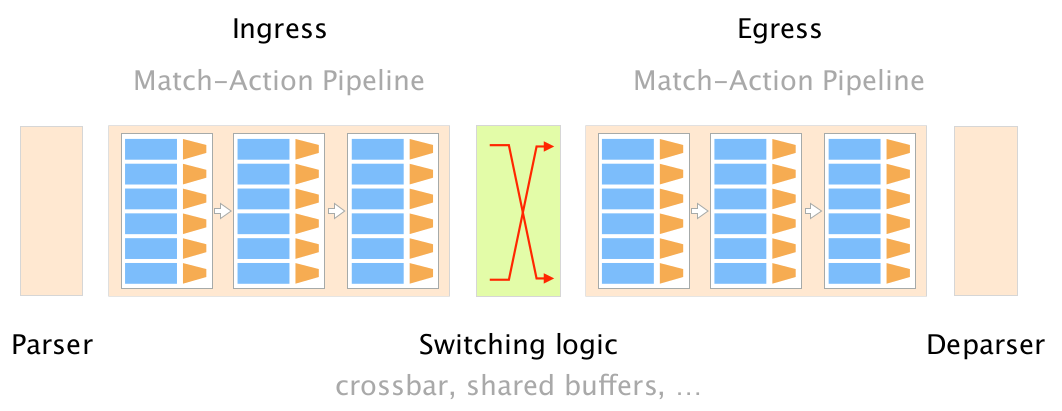
\includegraphics[width=0.75\textwidth,scale=1]{figures/PISA}
	\caption{Protocol Independent Switch Architecture (PISA) for high-speed programmable packet forwarding. \cite{advnet}}
	\label{fig:PISA}
\end{figure}

\newpage

\begin{figure}%[hb]
	\centering
	\begin{subfigure}[t]{.5\textwidth}
		\centering
		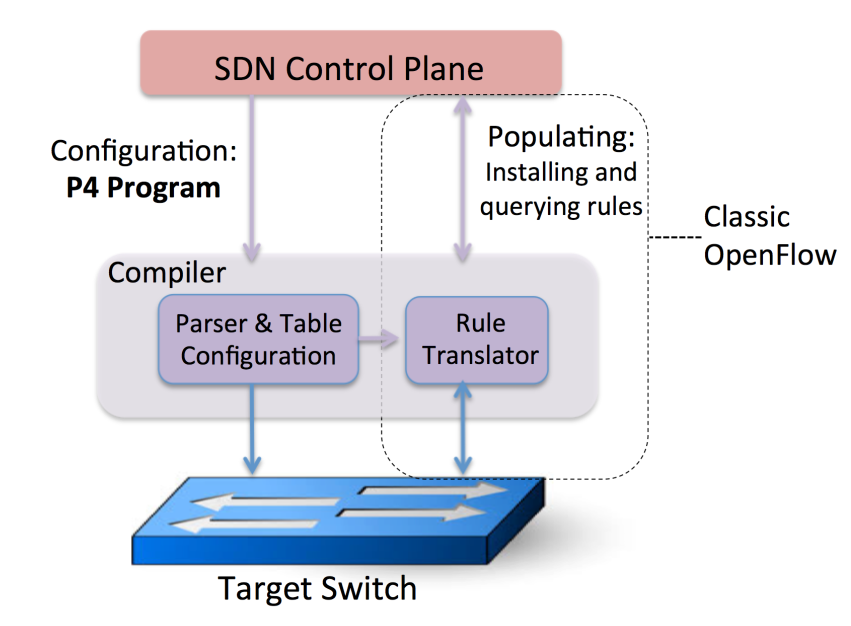
\includegraphics[width=\linewidth]{figures/P4_overview}
		\label{fig:P4_overview}
	\end{subfigure}%
	\begin{subfigure}[t]{.5\textwidth}
		\centering
		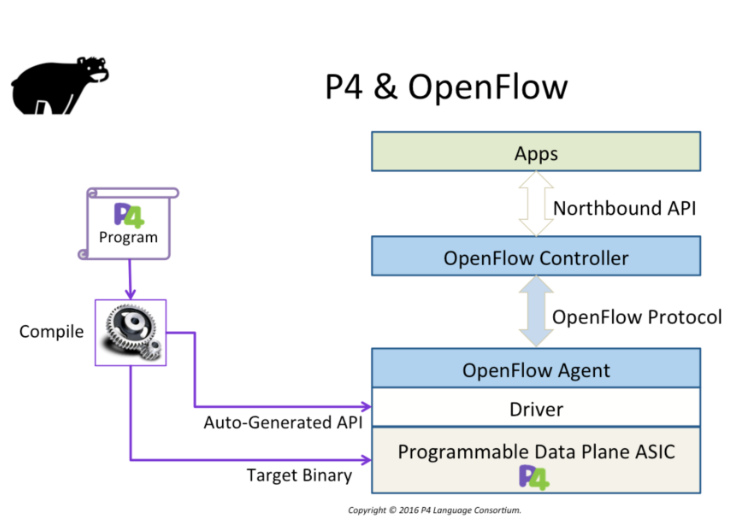
\includegraphics[width=\linewidth]{figures/P4_openflow}
		\label{fig:P4_openflow}
	\end{subfigure}
	\caption{P4 is a language to configure switches. \cite{bosshart2014p4}}
\end{figure}


Each chip has its own low-level interface, however this might vary for different hardware. Ideally we would want a higher-level language which can be used to configure a switch. This is exactly what P4 (Programming Protocol-independent Packet Processors) does: P4 is a higher-level language which is used to configure a switch, telling it how packets are to be processed. P4 can further be used with existing APIs (such as OpenFlow) that are designed to populate the forwarding tables in fixed function switches.














\label{lastpage} % this must stay here
\clearpage
\addcontentsline{toc}{section}{References}
\bibliographystyle{acm}
\bibliography{refs}

\clearpage
\appendix
\pagenumbering{Roman}

\end{document}
